\subsection{Video-in Port}
\label{sec:video_in}

The {\it \systemNameFull} includes a video-in port for use with the composite video-in
connector on the \DEBoard~board. The video analog-to-digital converter (ADC) connected to this
port is configured to support an NTSC video source. The video-in port provides frames of video 
at a resolution of 320 {\sf x} 240 pixels.  These video frames can be displayed on a 
monitor by using the video-out port described in Section~\ref{sec:video_out}.  The video-in 
port writes each frame of the video-in data into the pixel buffer described in 
Section~\ref{sec:pixel_buffer}. The video-in port can be configured to provide two types
of images: either the ``raw'' image provided by the video ADC, or a version of this image
in which only ``edges'' that are detected in the image are drawn.

The video-in port has a programming interface that consists of two registers, as
illustrated in Figure~\ref{fig:video_in}. The {\it Control} register at the address
{\sf 0xFF20306C} is used to enable or disable the video input. If the {\it EN} bit in this
register is set to 0, then the video-in core does not store any data into the pixel
buffer. Setting {\it EN} to 1 and then changing {\it EN} to 0 can be used to capture a 
still picture from the video-in port.

The register at address {\sf 0xFF203070} is used to enable or disable edge detection.
Setting the {\it E} bit in this register to 1 causes the input video to passed through
hardware circuits that detect edges in the images. The image stored in the pixel buffer
will then consist of dark areas that are punctuated by lighter lines along the edges that
have been detected.  Setting $E=0$ causes a normal image to be stored into the pixel
buffer.

\begin{figure}[h!]
   \begin{center}
       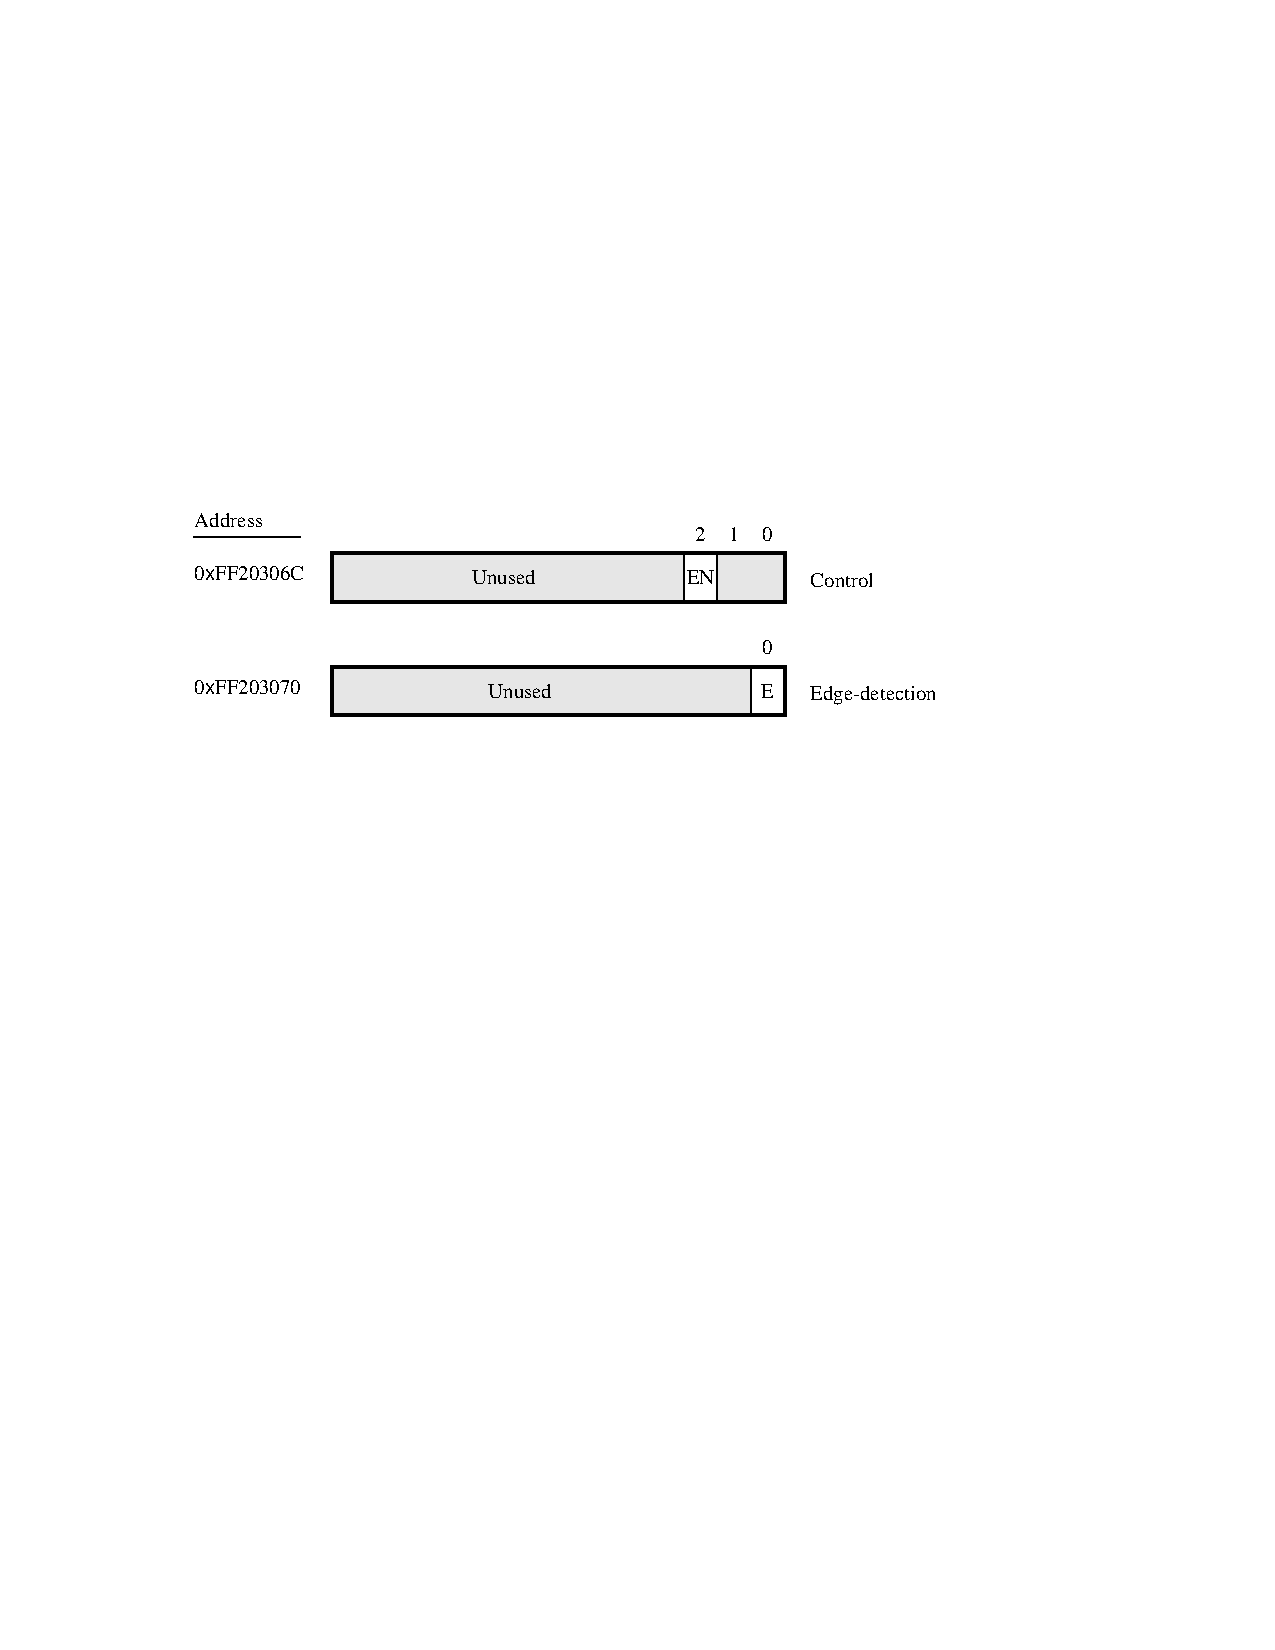
\includegraphics{../../../common/figs/Media_FPGA_Video_In.pdf}
   \end{center}
   \caption{The video-in port programming interface.}
	\label{fig:video_in}
\end{figure}

\subsubsection{DMA Controller for Video}
\label{sec:dma_video}

The data provided by the Video-In core is stored into memory using a DMA Controller for Video. When
operating in {\it Stream to Memory} mode, the DMA stores the incoming frames to memory. 
Table~\ref{tab:video_dma} describes the registers used in the DMA Controller.

\begin{table}[h]
    \centering
    \begin{tabular}{|c|l|c|c|c|c|c|c|c|c|c|c|}
        \hline
            \textbf{Address}
            & \multicolumn{1}{c|}{\textbf{Register}}
            & \multirow{2}{*}{\textbf{R/W}}
            & \multicolumn{9}{c|}{\textbf{Bit Description}}
        \\\cline{4-12}
            & \multicolumn{1}{c|}{\textbf{Name}}
            &
            & \textbf{31\ldots24}
            & \textbf{23\ldots16}
            & \textbf{15\ldots12}
            & \textbf{11\ldots8}
            & \textbf{7\ldots6}
            & \textbf{5\ldots3}
            & \textbf{2}
            & \textbf{1}
            & \textbf{0}
        \\\hline
            0xFF203060
            & \texttt{Buffer}
            & R
            & \multicolumn{9}{c|}{Buffer's start address}
        \\\hline
            0xFF203064
            & \texttt{BackBuffer}
            & R/W
            & \multicolumn{9}{c|}{Back buffer's start address}
        \\\hline
            0xFF203068
            & \texttt{Resolution}
            & R
            & \multicolumn{2}{c|}{Y}
            & \multicolumn{7}{c|}{X}
        \\\hline
            \multirow{2}{*}{0xFF20306C}
            & \texttt{Status}
            & R
            & m
            & n
            & {\footnotesize \it (1)}
            & BS
				& SB
            & {\footnotesize \it (1)}
            & EN
            & A
            & S
        \\\cline{2-12}

            & \texttt{Control}
            & W
            & \multicolumn{6}{c|}{\footnotesize \it (1)}
				& EN
            & \multicolumn{2}{c|}{\footnotesize \it (1)}
        \\\hline
                \multicolumn{11}{l}{}
        \\
                \multicolumn{11}{l}{\footnotesize \it{Notes: }}
        \\
                \multicolumn{11}{l}{\footnotesize{(1) Reserved. Read values are undefined. Write zero.}}
    \end{tabular}
		\caption{Video DMA Controller}
		\label{tab:video_dma}
\end{table}

The incoming video is stored to memory, starting at the address specified in the {\it Buffer} register. The 
{\it BackBuffer} register is used to store an alternate memory location. To change where the video is stored, 
the new location should first be written into the {\it BackBuffer}. Then the value in the {\it BackBuffer} and
{\it Buffer} registers can be switched by performing a write to the {\it Buffer} register. 

Bit 2 of the {\it Status/Control} register, {\it EN}, is used to enable or disable the Video DMA controller.
In the \systemName, the DMA controller is disabled by default. To enable the DMA controller, write a 
1 into this location. The Video DMA Controller will then begin storing the video into the location specified 
in the {\it Buffer} register.

The default value stored in the {\it Buffer} register is {\sf 0x08000000}. This address is also used as the 
source for the Video-Out port, as described in Section~\ref{sec:video_out}, allowing the Video In stream to be 
displayed on the VGA. If the Video-Out is intended to display a different signal, than the address stored in 
the Video DMA Controller's {\it Buffer} register should be changed. 
